\documentclass[12pt]{article}
\usepackage{fixltx2e}
\usepackage{float}
\newcommand{\degree}{\ensuremath{^\circ}}
\usepackage{graphicx}
\usepackage[margin=1.0in]{geometry}
\usepackage{amsmath}
\linespread{1.5}




\title{Portfolio Optimization in Python}
\author{Michael Lee \\*
The University of Texas at Austin}
\date{Fall 2013}

\begin{document}

\maketitle{}
Portfolio management can be viewed as an optimization problem in which profit is maximized subject to a limit on volatility. However, the proposed model choses instead to maximize expected utility (EU) via a monte carlo simulation. Randomly generated portfolio allocations are created and the EU of a risk-adverse investor is calculated to find the optimal portfolio. The price of each asset is pulled from online sources and is used to calculate both profit and volatility. Individual asset volatility is calculated using an exponentially-weighted moving average, which more strongly weights recent data, while the entire portfolio's volatility is calculated using traditional covariance. From historical data, each asset's future performance is predicted via linear regression. The locally optimal solution is defined as the portfolio with the highest EU without exceeding a predetermined level of risk. The model is run in the Python programming language and takes advantage of \emph{NumPy's} mathematical functions, \emph{Pandas} ability to handle time-series, as well as the \emph{Statsmodels'} statistical capabilities. 

\newpage
\section{The Base Model}
The original model as developed by Ruben Mercado, Scott Schwaitzberg, and David Kendrick utilizes a monte carlo method to randomly generate the stock prices. The performance of these stocks is simulated by the a random number generator times some coefficient. While this is pseudorandom, ultimately the asset's final price is determined by the hard-coded initial values. This is less than optimal, and misses the complexity that real data has to offer. Also, the covariance of the portfolio is not calculated, thus missing out on an important metric of portfolio diversification. 


\section{Improved Model in Python}
Building off the works of Mercado, Schwaitzberg, and Kendrick, an improved model is created. By instead maximizing expected utility of prices, the improved model more accurately simulate portfolio management. Historical data is used to predict future prices, transforming the model to a functional investment tool. The volatility of the entire portfolio is calculated using matrix operations to show the beneficial effects of diversification as suggested by Markowitz in his 1952 paper on Modern Portfolio Theory (Markowitz, 1990). Additionally, a more modern method of calculating asset volatility is built-in such that recent volatility is more heavily weighted. The proposed model retains the monte carlo method for optimization, as a closed form function could not be readily created.

\subsection{Expected Utility Function}
Mercado, Schwaitzberg, Kendrick, and I all initially maximized profit instead of utility. However, this oversimplification leads both our models to seek only the most profitable asset unless other constraints are placed. Expected utility factors in not only profitability ({\bf{${\pi}$}}), but the volatility of the asset, investor's level of risk-aversion ({\bf ${\beta}$}),  and the discount factor ({\bf {$\delta$}}). By using the EWMA instead of total volatility in EU calculations, the model simulates individuals' emphasis on recent events (i.e. failed product launch, law suites, etc.) when evaluating an asset's risk. 

\begin{equation}
	EU(\pi, EWMA, \beta, \delta, t) = 1 - \exp{(-\beta \frac{\pi}{EWMA} \delta^{t})}
\end{equation}

This functional form is based-off of the Arrow-Pratt measure of absolute risk-aversion (A) exhibiting constant risk-aversion (EconPort, 2013). 

\begin{equation}
	A(c) = -\frac{u''(c)}{u'(c)}
\end{equation}

\begin{figure}[H]
	\begin{center}
		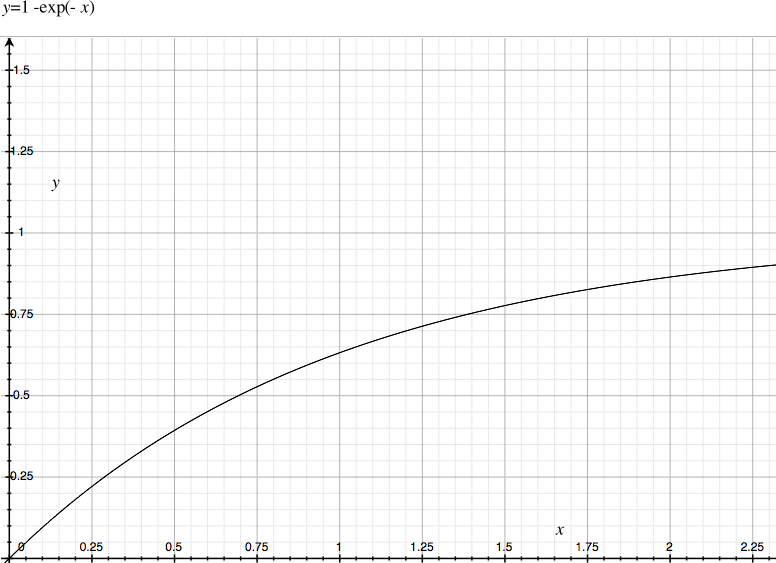
\includegraphics[scale=.4]{Figures/EU_fn.png}
		\caption{The Constant Risk-Averse Expected Utility Function}
	\end{center}
\end{figure}
Absolute risk-aversion (ABA) implies that the actor is equally averse to losing his first dollar as his hundredth and that risk-aversion is independent of wealth-- a property challenged by behavioral economists. Flaws aside, ABA functions are useful in modeling because of their simple derivatives and limit of one.  


\subsection{Pulling Real-Time Data}
Instead of simply creating fictional stock prices and volatility, the new model turns to the web for real world prices. By interfacing with Yahoo! Finance's API, we are able to pull historical financial data into the model, including the adjusted close price and ${\beta}$, a measure of an asset's covariance with the market (usually defined as the S\&P 500). ${\beta}$ is often used as a proxy for an asset's systemic risk, or the risk posed to all assets in a market segment and cannot be eliminated via portfolio diversification (\emph{LSE}). \\*\\*
From the historical data (01/01/2010 - Present), some basic statistics are calculated, including the mean (${\mu}$), standard deviation (${\sigma}$), and correlation (${\rho}$). Where ${\emph E}$ is the expected value operator:


\begin{equation}
	\mu = \frac{x_{1} + x_{2} ... + x_{n}} {n}
\end{equation}	

\begin{equation}
	\sigma = \sqrt{E[(X - \mu])^{2}}
\end{equation}	
	
\begin{equation}
	\rho_{x,y} = \frac{E(X - E[X])(Y-E[Y])}{\sigma_{x}\sigma_{y}}
\end{equation}

From the above we can evaluate how risky-- and profitable-- our portfolio is. The mean of the asset price over time is used to predict how profitable an asset will be; the standard deviation how volatile the asset is; the covariance how diversified our portfolio is. The covariance is particularly important in building a successful portfolio as it shows how the assets fluctuate in unison. A covariance of unity implies that the two assets move in equal amounts-- when the price of one increases the price of the other increases by the same percentage-- a covariance of negative one implies that when the price of one asset increases, the other asset decreases by the same amount. In this model, and optimal total covariance is naught, meaning that the portfolio will perform well regardless of volatility in one particular asset.

\subsection{Portfolio Diversification}
Modern portfolio theory (MPT) is the mathematical foundation for much of today's investing strategies, especially with regards to diversification. MPT attempts to maximize the EU of a portfolio for a given level of risk by creating a portfolio consisting of various assets. The theory suggests that since an individual asset is normally distributed, by selecting assets whose performance is not positively correlated, a risk-adverse investor can effectively insulate him or herself from market shocks. When returns are plotted against standard deviation, there exists some efficient frontier outside ({\bf Figure 1}) of which no better returns can be gain for a given level of risk.  

\begin{figure}[H]
	\begin{center}
		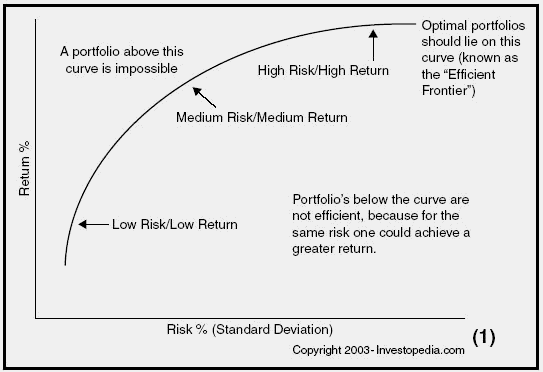
\includegraphics[scale=.75]{Figures/Efficient_Frontier.png}
		\caption{The Efficient Frontier}
	\end{center}
\end{figure}

With this concept in mind, we construct a metric of the portfolio's risk by relating each individual asset's volatility with its covariance with every other asset. For three assets:

\begin{equation}
	\Sigma = \sqrt{\sigma_{a} w_{a} + \sigma_{b} w_{b} + \sigma_{c} w{c} + ab*cov_{ab} + ac * cov_{ac} + bc cov_{vc} }`
\end{equation}

This is readily transformed into a matrix for any arbitrary number of assets. Thus, as the number of assets in the portfolio \emph{P} approaches infinity, the EU[\emph{P}] approaches the weighted mean of all constituent assets. 

\begin{equation} 
	\Sigma = 
	\begin{pmatrix} x_{1} & x_{2} & ... x_{n} \end{pmatrix}
	\begin{pmatrix} \sigma_{1} & \sigma_{12} & ... & \sigma_{1n} \\ 
	\sigma_{12} & \sigma_{2} & ... & \sigma_{2n} \\
	... & ... & ... & ... \\
	\sigma_{1n} & \sigma_{2n} & ... & \sigma_{nn} \end{pmatrix}
	\begin{pmatrix} x_{1} \\ x_{2} \\ ... \\ x_{n} \end{pmatrix}
\end{equation}

\* The above equation will result in a scalar value that will decrease in magnitude as the number of assets \emph{n} increases. MPT has been challenged in recent years as data has shown that many equities are not normally distributed, and instead have fatter tails, hence the phrase tail-side risk.

\subsection{Linear Regression and Forecasting}
In order to make the model a predictive tool for portfolio analysis and and not a sophisticated backwardization program, asset prices had to be forecasted into the future. To do this, linear regression was done on only the past six months of prices and from this data, forecasted  six months in the future. Data older than six months is disregarded as it has little influence on pricing in the short-term where fluctuations are dominated by asset and market momentum. \

Linear fitting is achieved by minimizing the sum of residuals between all points and the line of best fit. To accomplish this, the model employs a custom gradient (or steepest) decent algorithm. Where \emph{R} is the residual and \emph{m} is the slope:

\begin{equation}
	min: error = \frac{1}{m} * x^{T} * (x m - y)
\end{equation}




\subsection{Exponentially Weighted Moving Average}
While the standard mean is useful in understanding an asset's long-term value, it has major flaws in evaluating future success. An arithmetic mean equally weights recent and distant performance. This causes serious error in assets whose price has risen or fallen dramatically in recent times as an asset is more likely to follow current trends than distant trends. To account for this, an exponentially weighted moving average (EWMA) is taken for each asset. As described by Minkah (Minkah, 2007), the EWMA is defined as:

\begin{equation}
	\sigma = \sqrt{(1-\lambda) \sum{ \lambda^{i}(r_{i-1} - r_{avg})^2})}
\end{equation}

Where \emph{r} is the return on an asset and $\lambda$ is some decay factor. A financial services company, \emph{RiskMetrics}, as does this model, uses a decay factor of .94 to forecast. However, $\lambda$ can be changed to reflect the manager's opinion on how distant performance reflects future gains. 

\subsection{Monte Carlo Simulation}
Monte Carlo simulations are often used in financial modeling in situations where a closed-form analytic solution is not readily available or exceedingly computationally intensive. A monte carlo simulation relies on repeated random sampling of input variables to obtain an optimal result. In the case of portfolio management, by randomly choosing the asset allocation percentages and calculating the profit and volatility repeatedly, the law of averages states that as the number of simulations approaches infinity, an optimal solution will be found. \\*
In the proposed model, sampling was done according to the Dirichlet distribution, which ensures that some number of points, \emph{n}, are randomly sampled such that their sum is equal to some specified total. Thus, the Dirichlet distribution has the statistically appealing property of being the conjugate prior to the parameters of the multinomial distribution. 

\begin{equation}
	p({\bf p}) = Dirichlet({\bf p, u}) = \frac{1}{Z({\bf u})} \Pi p_{i}^{u_{i}-1}
\end{equation}

\subsection{Defining Optimality}
After repeated random sampling we will have a \emph{m x n} matrix where \emph{n} is the number of runs and \emph{m} houses the variables of interest, namely EU, profit, EWMA, and the weights of each asset in the portfolio. Where $w^{j}$ is the weight of each $j^{th}$ asset:

\[optimal(EU, \sigma) = \left | \begin{array}{ccc}
\pi_{1} & ... & \pi_{n} \\
\sigma_{1} & ... & \sigma_{n} \\
w_{1}^{1}  & ... & w_{1}^{n} \\
w_{2}^{1}  & ... & w_{2}^{n} \\
... & ... & ... \\
w_{j}^{1}  & ... & w_{j}^{n} \end{array} \right |\]

\* The optimal portfolio is the one that has the highest EU as defined by {{\bf equation 1}. 
\* However, a good portfolio will also limit the amount of exposure it has to market volatility. Thus, any portfolio allocation whose combined volatility--as defined by {\bf equation 7}-- is greater than a predefined level of risk is eliminated from the maximization. The optimization problem is now defined as:

\begin{equation}
	\begin{split} 
		& max: EU \\ 
		& s.t: \Sigma < \Sigma^{max}
	\end{split}
\end{equation}

The algorithm is designed such that the asset data is pulled once, and the allocation is run \emph{n} times. After the final matrix has been compiled, a search function is first used to eliminate all columns that do not satisfy {\bf equation 7}, then finally to find the column housing maximum profit. For a more detailed look at the full program, consult the appendix. 

\section{Results}
The monte carlo simulation was run 200 times at different values of $\beta$. All results were normalize to buying one share. \\*

A plot of the profit vs. the portfolio volatility is pictured below. The model conforms to was is predicted by MPT: many of the low-risk portfolios are also the lowest performing. We can infer from this relationship that as the investor's risk tolerance increases, he will be able to achieve higher returns by moving rightward on the plot. This is confirmed when we compare profits of optimal portfolios as functions of $\beta$. 

\begin{figure}[H]
\begin{center}
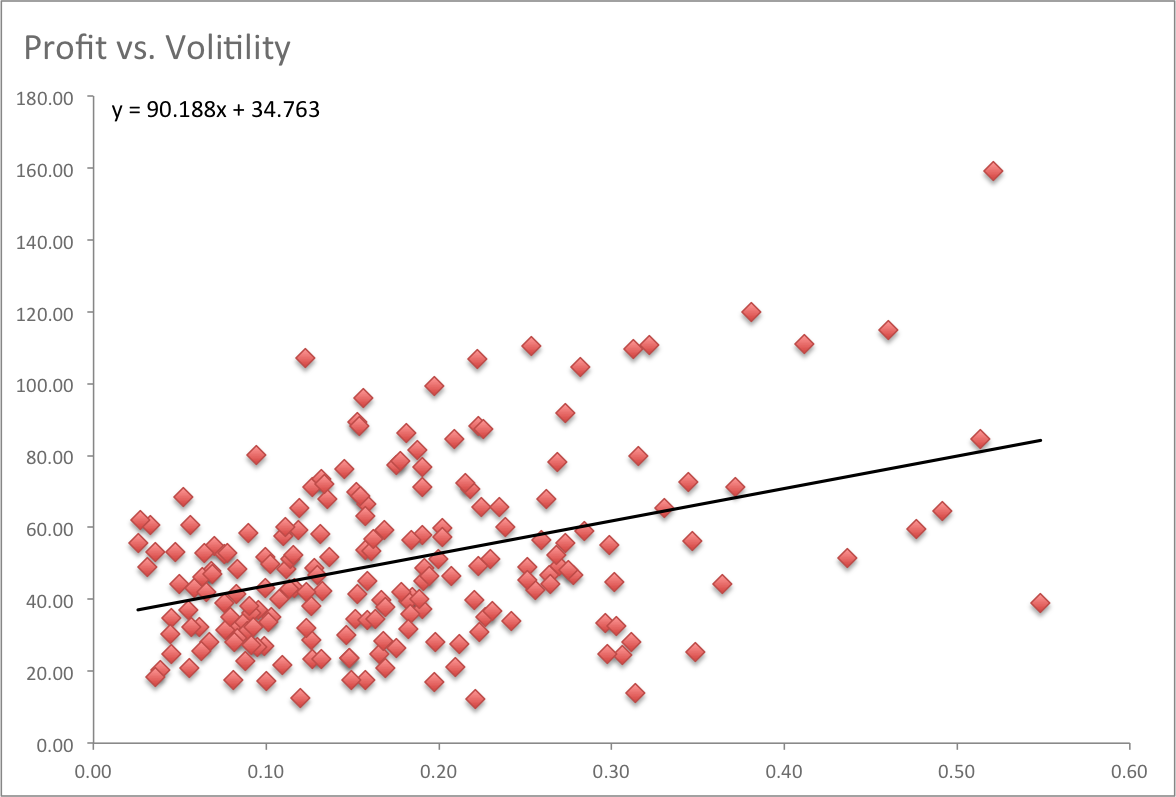
\includegraphics[scale=.6]{Figures/Profit_v_Volit.png}
\caption{Profit vs. Portfilio Volatility, $\beta = .8$}
\end{center}
\end{figure}

\begin{figure}[H]
\begin{center}
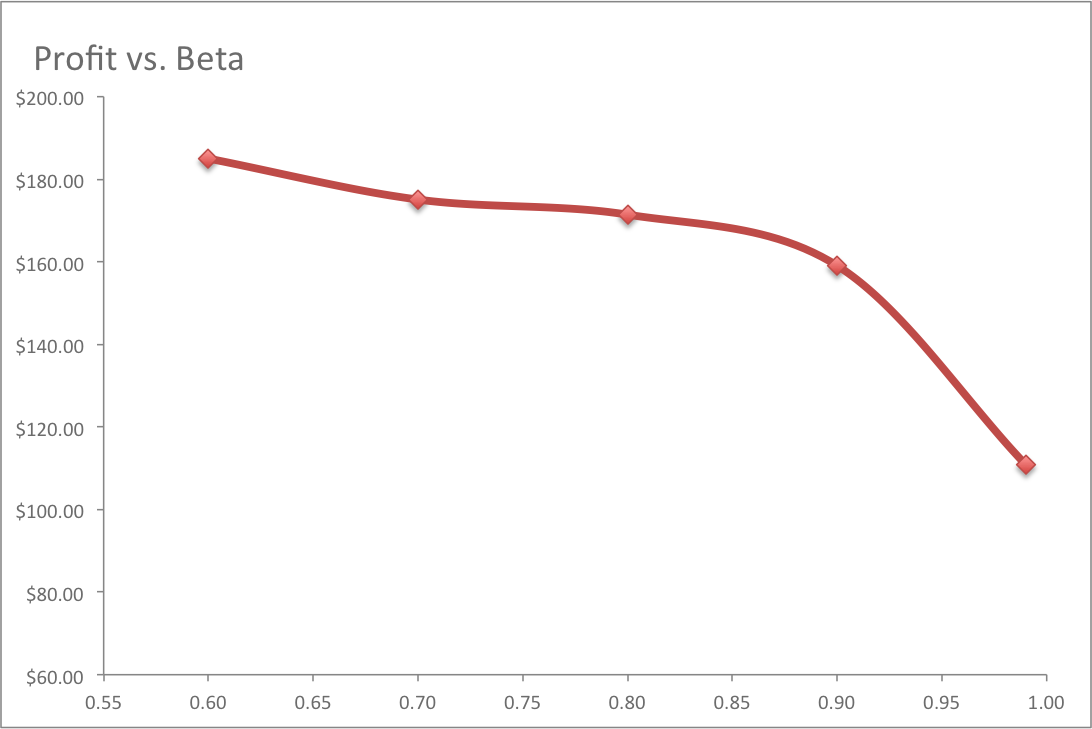
\includegraphics[scale=.6]{Figures/profit_v_beta.png}
\caption{Profit vs. Risk-tolerance}
\end{center}
\end{figure}


Since the EU is inversely related volatility and positively correlated with profit, there can exist multiple optimal solutions based on the criteria selected-- the portfolio with the highest EU is not necessarily the portfolio with the highest profit as seen below. 

\begin{figure}[H]
\begin{center}
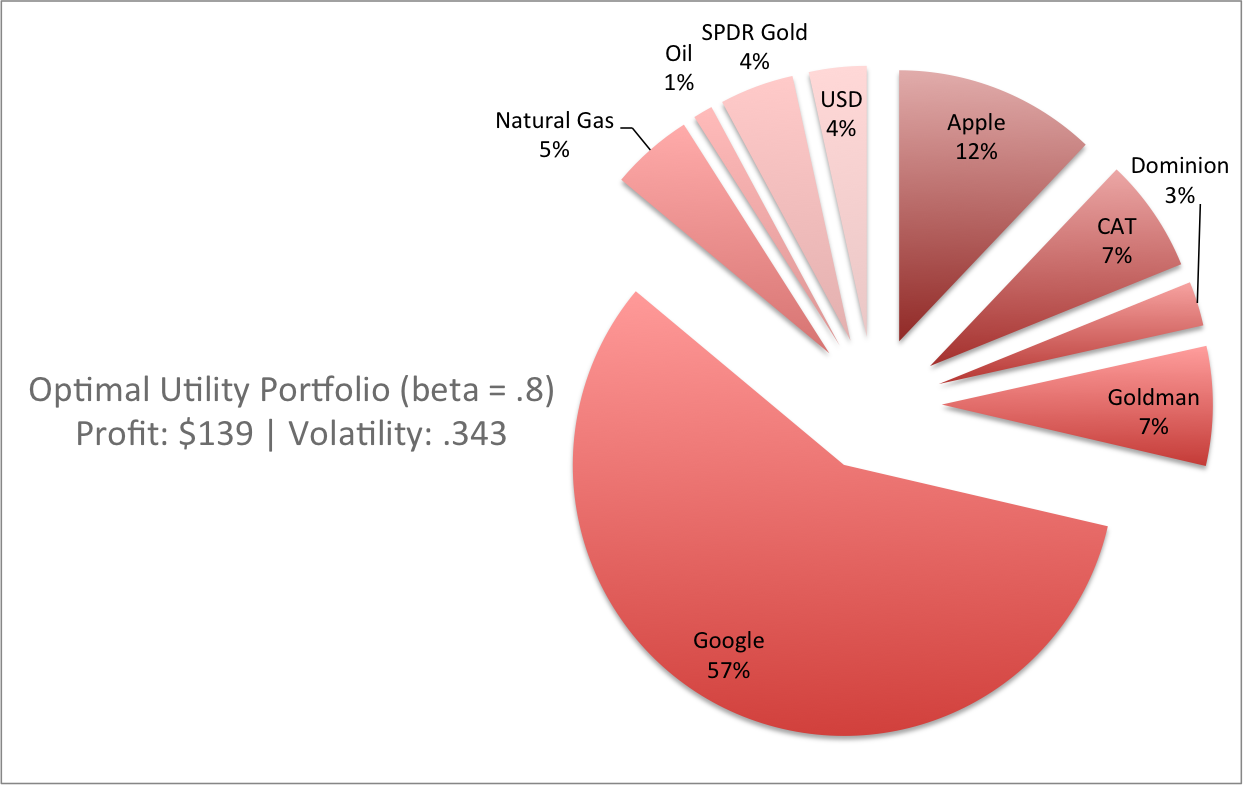
\includegraphics[scale=.75]{Figures/OptimalPort_EU.png}
\caption{The Optimal Portfolio Allocation Based on EU}
\end{center}
\end{figure}

When compared to the optimal portfolio determined by profit, the shift towards higher returns in riskier assets is evident. The model predicts an optimal portfolio with higher percentages of Google and Apple, with a smaller portion of safe assets such as the United States Dollar and gold.

\begin{figure}[H]
\begin{center}
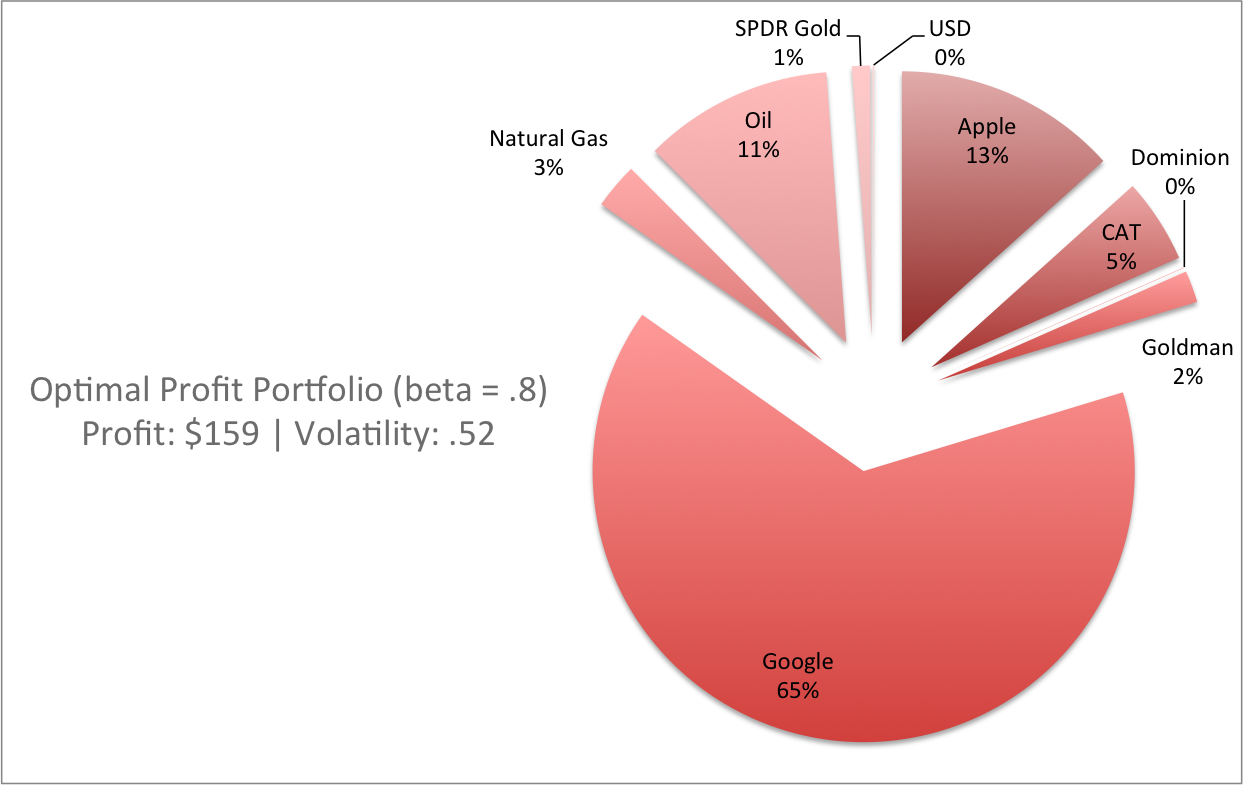
\includegraphics[scale=.75]{Figures/OptimalPort_profit.png}
\caption{The Optimal Portfolio Allocation Based on Profit}
\end{center}
\end{figure}


\*Another experiment was run to show the effect that investor risk-tolerance plays in selecting the optimal portfolio. Intuitively, an investor who is more risk-averse ({ modeled by a higher $\beta$}) will select a portfolio consisting of low-risk stocks. In the model, an asset is considered high-risk if its standard deviation is greater than \$20. By varying $\beta$ and observing the effect on the optimal portfolio, we can confirm if the model matches intuition. 

\begin{figure}[H]
\begin{center}
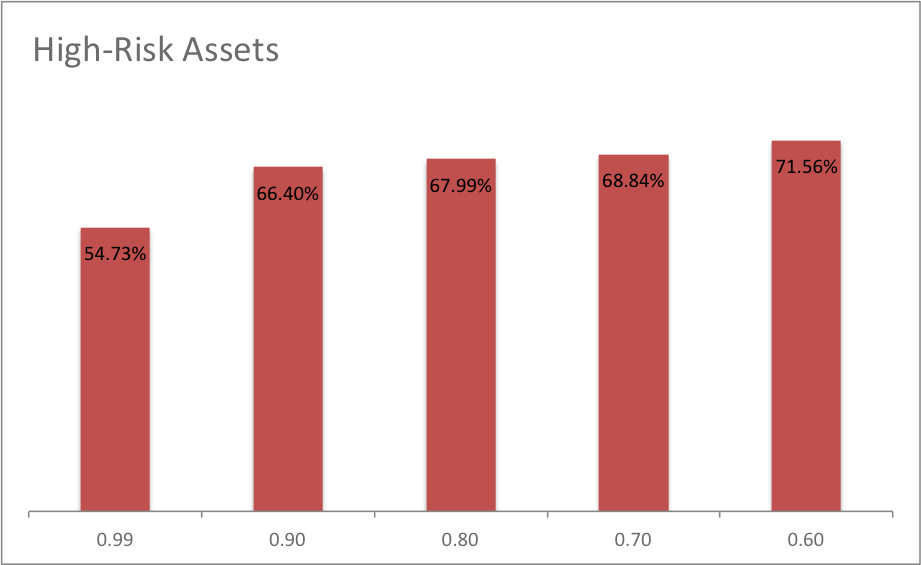
\includegraphics[scale=1]{Figures/High_Risk.png}
\caption{High-Risk Assets in the Optimal Portfolio}
\end{center}
\end{figure}


\section{Future Improvements}
Given more time, the model can be improved to become a better forecasting agent by creating a Markov chain in which the asset’s future performance can be predicted based on deterministic processes. This would allow the model to not only select optimal allocations based on a long-term view, but enable shorting based on the stochastic probabilities of tomorrow’s events. \\*
Future iterations of the model can be altered to incorporate non-traditional assets, such as options and derivatives via the Black-Scholes equation. This would allow for a more robust portfolio as these assets have characteristics such as a negative beta, i.e. that they perform well when the market doesn't. \\* 

\newpage
\section{Appendix}

\subsection{Normalized Asset Performance}
\begin{figure}[H]
	\begin{center}
		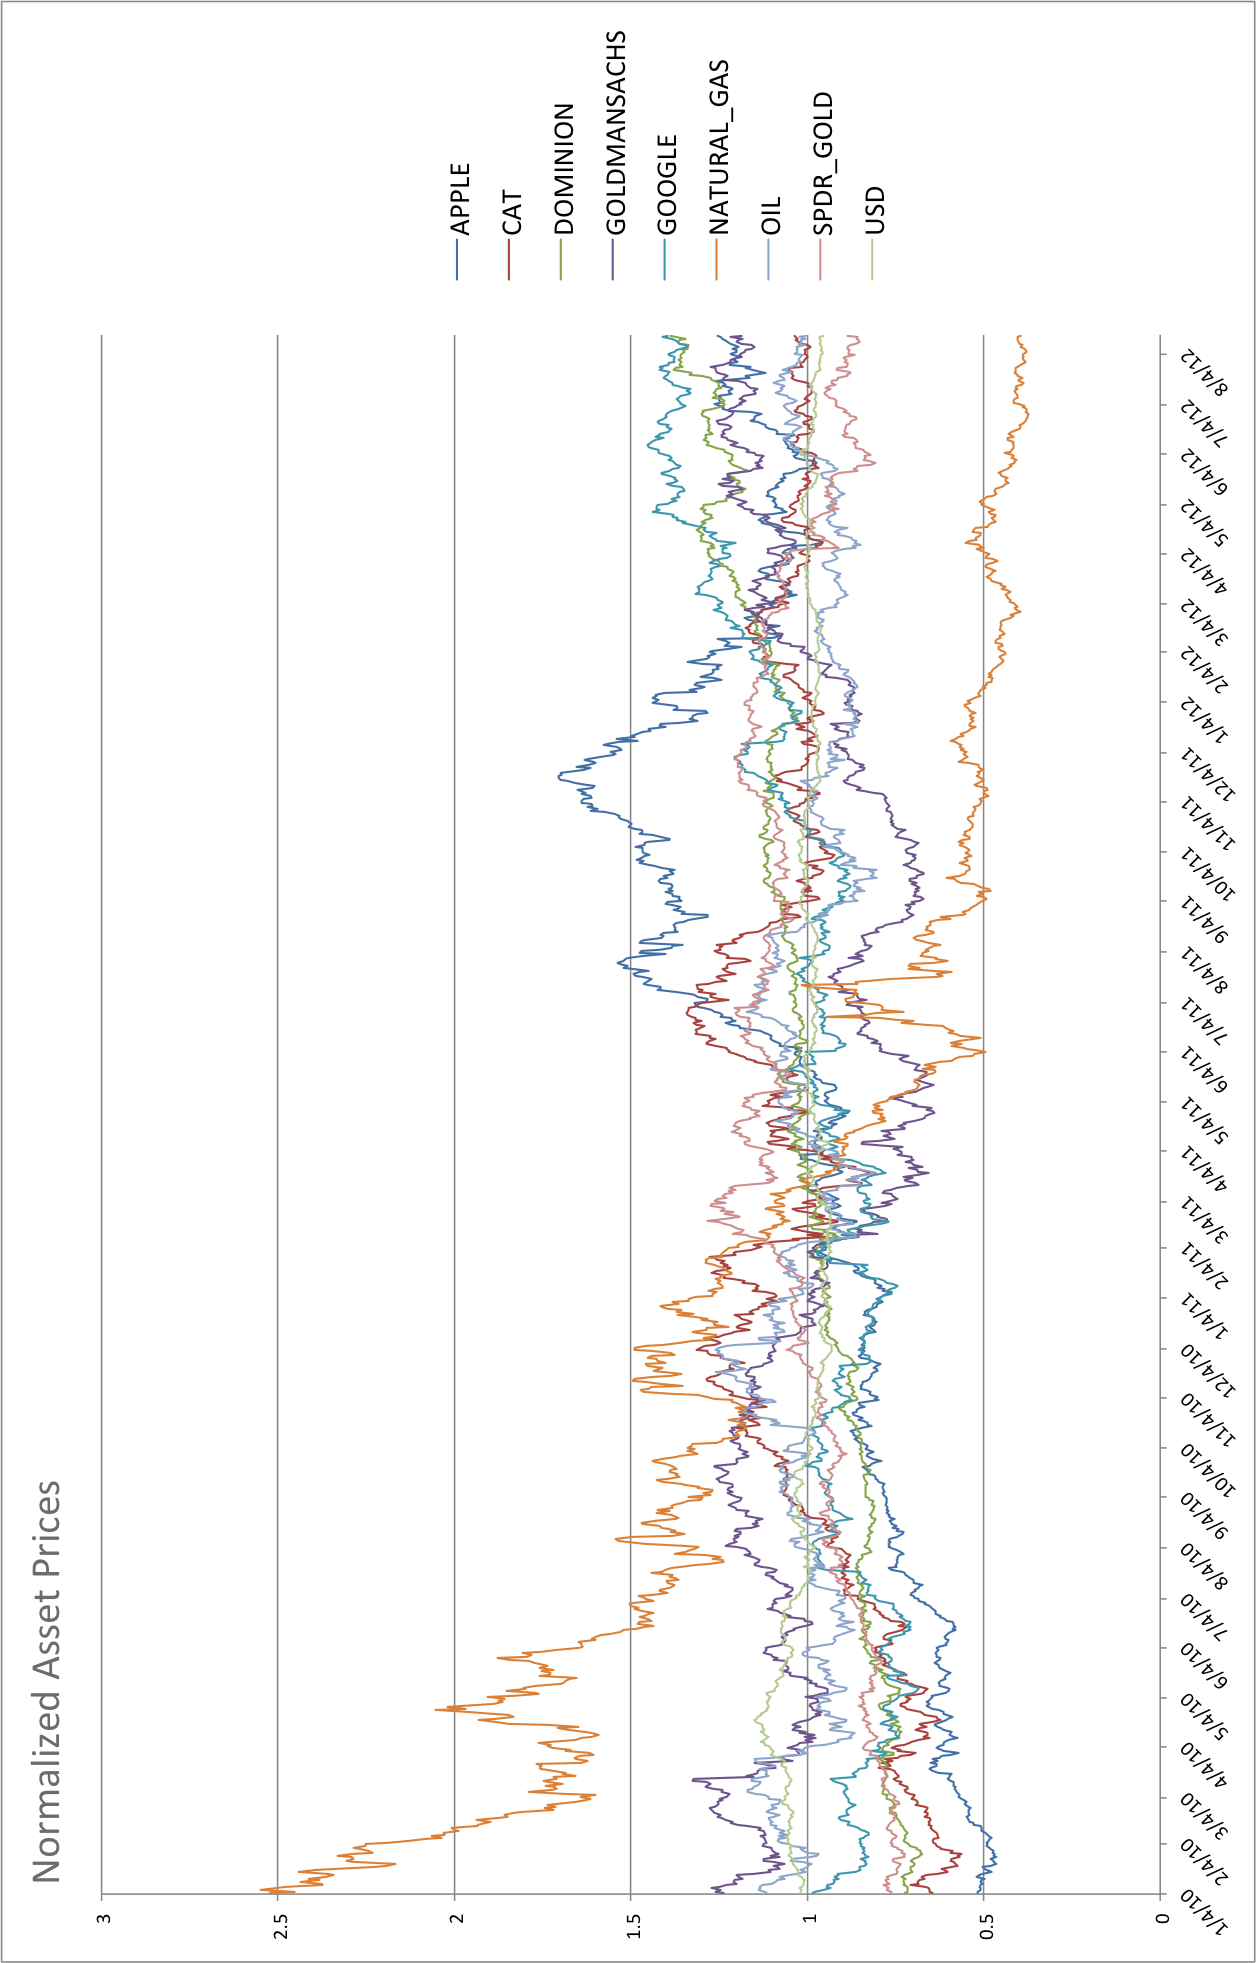
\includegraphics[scale=.6]{Figures/assets.png}
		\caption{Normalized Asset Performance Since 2010}
	\end{center}
\end{figure}



\end{document}
